% SATE Therapy Data Tracking — Example (session 6 of 8, follows SATE-Therapy_Plan.tex)
% Compile with: pdflatex -output-directory=build SATE-Therapy_Data_Tracking.tex (run twice)
\documentclass[10pt,a4paper]{article}

% ---------- Fonts: serif body + sans headings/labels ----------
\usepackage[T1]{fontenc}
\usepackage[utf8]{inputenc}
\usepackage{mathpazo}
\usepackage[scaled=0.90]{helvet}
\usepackage{microtype}

% ---------- Layout (tight, single page) ----------
\usepackage[a4paper,top=0.8cm,bottom=0.85cm,left=1.4cm,right=1.4cm]{geometry}
\linespread{0.95}
\setlength{\parindent}{0pt}
\setlength{\parskip}{2pt}

% ---------- Color theme (shared SATE style) ----------
\usepackage[table,dvipsnames]{xcolor}
\definecolor{accent}{HTML}{215C68}
\definecolor{accentlt}{HTML}{9CC3CB}
\definecolor{goalgreen}{HTML}{2E7D4F}
\definecolor{amber}{HTML}{B8860B}
\definecolor{concern}{HTML}{B03A2E}
\definecolor{mono}{HTML}{6E6E6E}
\definecolor{fog}{HTML}{6E6E6E}

% ---------- Tables ----------
\usepackage{booktabs}
\usepackage{tabularx}
\usepackage{array}
\usepackage{multirow}
\renewcommand{\arraystretch}{1.02}

% ---------- Graphics / boxes ----------
\usepackage{tikz}
\usepackage[most]{tcolorbox}

% Goal box: colored left border, color = goal color
\newtcolorbox{goalbox}[1]{enhanced,colback=#1!5,colframe=#1!5,
  borderline west={2.5pt}{0pt}{#1},arc=1.5pt,
  left=6pt,right=6pt,top=3pt,bottom=3pt,boxsep=0pt,before skip=2.5pt,after skip=2pt}
% Note box: amber left border
\newtcolorbox{notebox}{enhanced,colback=amber!6,colframe=amber!6,
  borderline west={2.5pt}{0pt}{amber!80},arc=1.5pt,
  left=6pt,right=6pt,top=3pt,bottom=3pt,boxsep=0pt,before skip=3pt,after skip=3pt}

% ---------- Badges (rounded pills) ----------
\newcommand{\badge}[2]{\tcbox[on line,boxrule=0.4pt,arc=4pt,left=3pt,right=3pt,
  top=0.8pt,bottom=0.8pt,boxsep=0pt,colback=#1!13,colframe=#1!55!black!55]
  {\sffamily\scriptsize\bfseries\textcolor{#1!40!black}{#2}}}
\newcommand{\bEX}{\badge{mono}{EXAMPLE}}

% ---------- Goal chips (tiny pills, color-coded per goal) ----------
\newcommand{\gchip}[2]{\tcbox[on line,boxrule=0.4pt,arc=3.5pt,left=2.5pt,right=2.5pt,
  top=0.5pt,bottom=0.5pt,boxsep=0pt,colback=#1!12,colframe=#1!50!black!50]
  {\sffamily\fontsize{6}{6}\selectfont\bfseries\textcolor{#1!35!black}{#2}}}
\newcommand{\gA}[1]{\gchip{accent}{#1}}     % Goal 1 morphosyntax
\newcommand{\gB}[1]{\gchip{goalgreen}{#1}}  % Goal 2 vocabulary
\newcommand{\gC}[1]{\gchip{amber}{#1}}      % Goal 3 articulation

% ---------- Section styling ----------
\usepackage{pifont}
\usepackage{titlesec}
\setcounter{secnumdepth}{0}
\titleformat{\section}[block]{\sffamily\bfseries\small}{}{0pt}
  {\textcolor{accent}{\rule[-2.5pt]{2.5pt}{10.5pt}}\hspace{0.55em}\color{accent}\textls[70]}
\titlespacing*{\section}{0pt}{0.5em}{0.2em}

% ---------- Info-bar field ----------
\newcommand{\infofield}[2]{{\sffamily\fontsize{5.5}{6.5}\selectfont\color{black!55}\textls[50]{#1}}\hspace{0.35em}{\small #2}}

% ---------- Trend-chart helpers ----------
% y tick label at height #1 (y units), text #2
\newcommand{\ytick}[2]{\node[anchor=east,font=\sffamily\fontsize{5}{5}\selectfont,text=fog] at (0.72,#1) {#2};}

% ---------- Inline bars ----------
% Stacked support-mix bar: #1 color, #2 dark frac (indep./spont.), #3 light frac (cued/prompted); rest gray
\newcommand{\mixbar}[3]{\begin{tikzpicture}[baseline=-0.6pt]
  \pgfmathsetmacro{\tmpa}{#2*1.3}
  \pgfmathsetmacro{\tmpb}{(#2+#3)*1.3}
  \fill[gray!22,rounded corners=1pt] (0,0) rectangle (1.3,0.15);
  \fill[#1!45,rounded corners=1pt] (0,0) rectangle (\tmpb,0.15);
  \fill[#1,rounded corners=1pt] (0,0) rectangle (\tmpa,0.15);
  \ifdim \tmpa cm > 0.02cm \draw[white,line width=0.5pt] (\tmpa,-0.012) -- (\tmpa,0.162); \fi
  \ifdim \tmpb cm > 0.02cm \ifdim \tmpb cm < 1.28cm \draw[white,line width=0.5pt] (\tmpb,-0.012) -- (\tmpb,0.162); \fi\fi
\end{tikzpicture}}
% Bullet accuracy bar: #1 color, #2 frac, #3 target frac (dark notch)
\newcommand{\accbar}[3]{\begin{tikzpicture}[baseline=-0.6pt]
  \pgfmathsetmacro{\tmpa}{#2*1.3}
  \pgfmathsetmacro{\tmpt}{#3*1.3}
  \fill[gray!22,rounded corners=1pt] (0,0) rectangle (1.3,0.15);
  \fill[#1,rounded corners=1pt] (0,0) rectangle (\tmpa,0.15);
  \draw[black!50,line width=0.6pt] (\tmpt,-0.045) -- (\tmpt,0.195);
\end{tikzpicture}}
% Wide tile progress bar: #1 color, #2 frac, #3 target frac
\newcommand{\tilebar}[3]{\begin{tikzpicture}[baseline=-0.6pt]
  \pgfmathsetmacro{\tmpa}{#2*4.6}
  \pgfmathsetmacro{\tmpt}{#3*4.6}
  \fill[gray!20,rounded corners=1.2pt] (0,0) rectangle (4.6,0.18);
  \fill[#1,rounded corners=1.2pt] (0,0) rectangle (\tmpa,0.18);
  \draw[black!50,line width=0.7pt] (\tmpt,-0.05) -- (\tmpt,0.23);
\end{tikzpicture}}

\usepackage[hidelinks]{hyperref}
\pagestyle{empty}

\begin{document}

% ================= Header =================
\noindent
\begin{minipage}[b]{0.62\linewidth}
{\sffamily\LARGE\bfseries\color{accent} SATE - Therapy Data Tracking}\hspace{0.6em}\raisebox{2.5pt}{\bEX}
\end{minipage}\hfill
\begin{minipage}[b]{0.36\linewidth}\raggedleft
{\sffamily\scriptsize\color{black!65}Date: 2026--07--23\quad Clinician: \rule[-1pt]{1.6cm}{0.3pt}\\[1pt]
Basis: session 6 audio (SATE Record) $\cdot$ SATE - Therapy Plan}
\end{minipage}
\\[2pt]
{\color{accentlt}\rule{\linewidth}{1pt}}

% ---------- Session info bar ----------
\vspace{1.5pt}
\begin{tcolorbox}[colback=gray!5,colframe=gray!25,boxrule=0.4pt,arc=2pt,
  left=6pt,right=6pt,top=2.5pt,bottom=2.5pt,boxsep=0pt]
\infofield{CLIENT}{Child (C)}\quad
\infofield{AGE}{6;6}\quad
\infofield{SESSION}{6 of 8}\quad
\infofield{RECORDING}{45 min}
\end{tcolorbox}

% ---------- At-a-glance tiles ----------
\vspace{1pt}
\noindent
\begin{minipage}[t]{0.323\linewidth}
\begin{tcolorbox}[enhanced,colback=accent!4,colframe=accent!4,
  borderline west={2.5pt}{0pt}{accent},arc=1.5pt,
  left=6pt,right=6pt,top=2.5pt,bottom=2.5pt,boxsep=0pt]
{\sffamily\fontsize{5.5}{6}\selectfont\bfseries\color{black!55}\textls[60]{GOAL 1 · TENSE \& AGREEMENT}}\hfill\badge{goalgreen}{ON TRACK}\\[2pt]
{\sffamily\fontsize{14}{14}\selectfont\bfseries\color{black!80}63\%}{\sffamily\scriptsize\color{black!55}\ indep.\ this session}\hfill{\sffamily\scriptsize\bfseries\color{goalgreen}\ding{115}\,+8}\\[3pt]
\tilebar{accent}{0.63}{0.80}\\[1pt]
{\sffamily\fontsize{5.5}{6}\selectfont\color{black!45}baseline 0\%\hfill target 80\% (S8)}
\end{tcolorbox}
\end{minipage}\hfill
\begin{minipage}[t]{0.323\linewidth}
\begin{tcolorbox}[enhanced,colback=goalgreen!4,colframe=goalgreen!4,
  borderline west={2.5pt}{0pt}{goalgreen},arc=1.5pt,
  left=6pt,right=6pt,top=2.5pt,bottom=2.5pt,boxsep=0pt]
{\sffamily\fontsize{5.5}{6}\selectfont\bfseries\color{black!55}\textls[60]{GOAL 2 · VOCABULARY}}\hfill\badge{goalgreen}{ON TRACK}\\[2pt]
{\sffamily\fontsize{14}{14}\selectfont\bfseries\color{black!80}8\,/\,10}{\sffamily\scriptsize\color{black!55}\ words spont.\ (cum.)}\hfill{\sffamily\scriptsize\bfseries\color{goalgreen}\ding{115}\,+1}\\[3pt]
\tilebar{goalgreen}{0.80}{0.99}\\[1pt]
{\sffamily\fontsize{5.5}{6}\selectfont\color{black!45}baseline 0\hfill target 10 (S8)}
\end{tcolorbox}
\end{minipage}\hfill
\begin{minipage}[t]{0.323\linewidth}
\begin{tcolorbox}[enhanced,colback=amber!4,colframe=amber!4,
  borderline west={2.5pt}{0pt}{amber},arc=1.5pt,
  left=6pt,right=6pt,top=2.5pt,bottom=2.5pt,boxsep=0pt]
{\sffamily\fontsize{5.5}{6}\selectfont\bfseries\color{black!55}\textls[60]{GOAL 3 · ARTICULATION /s/}}\hfill\badge{amber}{WATCH}\\[2pt]
{\sffamily\fontsize{14}{14}\selectfont\bfseries\color{black!80}55\%}{\sffamily\scriptsize\color{black!55}\ CVC words}\hfill{\sffamily\scriptsize\bfseries\color{goalgreen}\ding{115}\,+13}\\[3pt]
\tilebar{amber!80!black}{0.55}{0.80}\\[1pt]
{\sffamily\fontsize{5.5}{6}\selectfont\color{black!45}baseline 0\% (word level)\hfill target 80\% (S8)}
\end{tcolorbox}
\end{minipage}

% ================= 1. Session activities =================
\section{Session 6 Activities \hspace{0.4em}{\normalfont\sffamily\scriptsize\color{black!55}(as delivered; per SATE - Therapy Plan)}}

{\footnotesize
\ding{172} Book \emph{Froggy Gets Dressed}: shared reading, review clothing words \hfill\gB{2}\\
\ding{173} Paper-doll craft: narrate the outfit in 3rd person; /s/ CVC (\emph{sock, suit}) \hfill\gA{1}\,\gB{2}\,\gC{3}\\
\ding{174} ``Guess Who'' game: ``\textbf{He} ha\textbf{s} / she \textbf{is} wearing'' question frames \hfill\gA{1}}\\[-1pt]
{\scriptsize\itshape\color{black!55}All counts are auto-compiled from the session audio. Independent = no model in the preceding utterance; cued = $\leq$1 verbal model. Morphological \texttt{-s} is credited to Goal 1 even when /s/ is distorted --- no double penalty.}

% ================= 2. Goal performance =================
\section{Goal Performance \hspace{0.4em}{\normalfont\sffamily\scriptsize\color{black!55}(bars: \textbf{dark} = independent/spontaneous $\cdot$ \textbf{light} = cued/prompted $\cdot$ gray = missed; notch = target $\cdot$ charts: S1--S6, dashed = target, shaded = probe)}}

% ---- Goal 1 ----
\begin{goalbox}{accent}
{\sffamily\small\bfseries\color{accent} Goal 1 --- Tense \& agreement morphology}\hfill
{\sffamily\scriptsize\color{black!55}target 80\% independent by S8}\\[2pt]
\begin{minipage}[c]{0.675\linewidth}
\footnotesize\setlength{\tabcolsep}{2.2pt}
\begin{tabular}{@{}l r r r r r r l@{}}
\toprule
\rowcolor{accent!10}
{\sffamily\bfseries\scriptsize Target} & {\sffamily\bfseries\scriptsize Contexts} & {\sffamily\bfseries\scriptsize Independent} & {\sffamily\bfseries\scriptsize Cued} & {\sffamily\bfseries\scriptsize Missed} & {\sffamily\bfseries\scriptsize Independent\,\%} & {\sffamily\bfseries\scriptsize $\Delta$ vs.\ S5} & {\sffamily\bfseries\scriptsize Support mix}\\
\midrule
3rd-sg \texttt{-s} (STG 1a) & 14 & 9 & 3 & 2 & 64\% & \textcolor{goalgreen}{+6} & \mixbar{accent}{0.643}{0.214}\\
\arrayrulecolor{black!20}\midrule
\quad structured frames (\ding{174}) & 8 & 6 & 2 & 0 & 75\% & --- & \mixbar{accent}{0.75}{0.25}\\
\midrule
\quad spontaneous narration (\ding{173}) & 6 & 3 & 1 & 2 & 50\% & --- & \mixbar{accent}{0.50}{0.167}\\
\midrule
copula/aux \emph{is} (STG 1b) & 10 & 6 & 3 & 1 & 60\% & \textcolor{goalgreen}{+8} & \mixbar{accent}{0.60}{0.30}\\
\midrule
\textbf{Combined} & \textbf{24} & \textbf{15} & \textbf{6} & \textbf{3} & \textbf{63\%} & \textcolor{goalgreen}{\textbf{+8}} & \mixbar{accent}{0.625}{0.25}\\
\arrayrulecolor{black}\bottomrule
\end{tabular}\\[1.5pt]
{\scriptsize\itshape\color{black!55}Accuracy with $\leq$1 cue (dark+light): 88\% combined. First spontaneous ``He has\,...'' frames in \ding{174}; cues faded from gesture+verbal (S1--S3) to verbal only; all 3 misses were omissions (no overgeneralization).}
\end{minipage}\hfill
\begin{minipage}[c]{0.295\linewidth}\centering
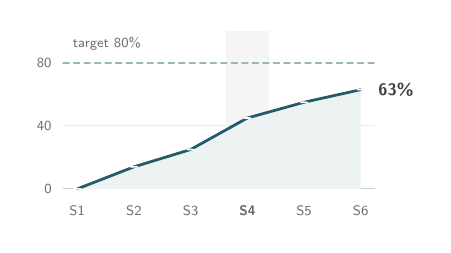
\begin{tikzpicture}[x=0.72cm,y=0.02cm,line cap=round,line join=round]
  \fill[black!4] (3.62,0) rectangle (4.38,100);
  \draw[gray!15,line width=0.3pt] (0.75,40) -- (6.25,40);
  \draw[accent!45,line width=0.5pt,dash pattern=on 2.2pt off 1.6pt] (0.75,80) -- (6.25,80);
  \draw[gray!40,line width=0.4pt] (0.75,0) -- (6.25,0);
  \ytick{0}{0}\ytick{40}{40}\ytick{80}{80}
  \node[anchor=south west,font=\sffamily\fontsize{5}{5}\selectfont,text=fog] at (0.75,82) {target 80\%};
  \fill[accent!8] (1,0) -- (2,14) -- (3,25) -- (4,45) -- (5,55) -- (6,63) -- (6,0) -- cycle;
  \draw[accent,line width=1pt] (1,0)--(2,14)--(3,25)--(4,45)--(5,55)--(6,63);
  \foreach \s/\v in {1/0,2/14,3/25,4/45,5/55,6/63}{\filldraw[fill=accent,draw=white,line width=0.5pt] (\s,\v) circle (0.062);}
  \node[anchor=west,font=\sffamily\fontsize{6}{6}\selectfont\bfseries,text=black!75] at (6.14,63) {63\%};
  \foreach \s in {1,2,3,5,6}{\node[anchor=north,yshift=-2.5pt,font=\sffamily\fontsize{5}{5}\selectfont,text=fog] at (\s,0) {S\s};}
  \node[anchor=north,yshift=-2.5pt,font=\sffamily\fontsize{5}{5}\selectfont\bfseries,text=black!60] at (4,0) {S4};
\end{tikzpicture}\\[0.5pt]
{\scriptsize\color{fog}combined independent accuracy}
\end{minipage}
\end{goalbox}

% ---- Goal 2 ----
\begin{goalbox}{goalgreen}
{\sffamily\small\bfseries\color{goalgreen} Goal 2 --- Expressive vocabulary}\hfill
{\sffamily\scriptsize\color{black!55}target 10 spontaneous theme words by S8}\\[2pt]
\begin{minipage}[c]{0.67\linewidth}
\footnotesize\setlength{\tabcolsep}{2.5pt}
\begin{tabular}{@{}l l r r r l l@{}}
\toprule
\rowcolor{goalgreen!10}
{\sffamily\bfseries\scriptsize Word} & {\sffamily\bfseries\scriptsize New/review} & {\sffamily\bfseries\scriptsize Models} & {\sffamily\bfseries\scriptsize Produced} & {\sffamily\bfseries\scriptsize Spontaneous} & {\sffamily\bfseries\scriptsize Support mix} & {\sffamily\bfseries\scriptsize Best use}\\
\midrule
\emph{sock} & new & 6 & 4 & 2 & \mixbar{goalgreen}{0.333}{0.333} & \gchip{goalgreen}{SPONT}\\
\arrayrulecolor{black!20}\midrule
\emph{suit} & new & 5 & 2 & 0 & \mixbar{goalgreen}{0}{0.40} & \gchip{amber}{PROMPT}\\
\midrule
\emph{hat} & review & 4 & 4 & 3 & \mixbar{goalgreen}{0.75}{0.25} & \gchip{goalgreen}{SPONT}\\
\midrule
\emph{zip} & review & 5 & 3 & 2 & \mixbar{goalgreen}{0.40}{0.20} & \gchip{goalgreen}{SPONT}\\
\midrule
\emph{shirt} & review & 4 & 3 & 0 & \mixbar{goalgreen}{0}{0.75} & \gchip{amber}{PROMPT}\\
\midrule
\emph{pants} & review & 3 & 2 & 0 & \mixbar{goalgreen}{0}{0.667} & \gchip{amber}{PROMPT}\\
\midrule
\emph{button} & review & 3 & 1 & 0 & \mixbar{goalgreen}{0}{0.333} & \gchip{concern}{IMIT}\\
\midrule
\textbf{Cumulative spontaneous} & & & & \textbf{8 / 10} & \accbar{goalgreen}{0.80}{0.99} & \textbf{80\% of LTG}\\
\arrayrulecolor{black}\bottomrule
\end{tabular}\\[1.5pt]
{\scriptsize\itshape\color{black!55}Spontaneous = no model in the preceding utterance (best: ``my sock is wet''). Cumulative = target words used spontaneously at least once (8 of 16 taught; LTG = 10). \emph{hat, shirt, pants} are review vocabulary; \emph{button} carried over to S7 review.}
\end{minipage}\hfill
\begin{minipage}[c]{0.30\linewidth}\centering
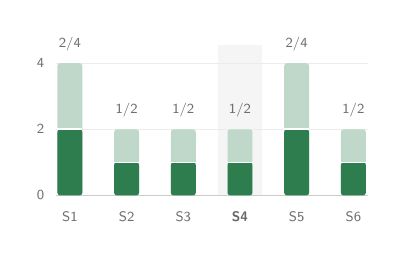
\begin{tikzpicture}[x=0.72cm,y=0.42cm]
  \fill[black!4] (3.62,0) rectangle (4.38,4.55);
  \draw[gray!15,line width=0.3pt] (0.75,2) -- (6.25,2);
  \draw[gray!15,line width=0.3pt] (0.75,4) -- (6.25,4);
  \draw[gray!40,line width=0.4pt] (0.75,0) -- (6.25,0);
  \ytick{0}{0}\ytick{2}{2}\ytick{4}{4}
  \foreach \s/\t/\m in {1/4/2,2/2/1,3/2/1,4/2/1,5/4/2,6/2/1}{
    \fill[goalgreen!30,rounded corners=1pt] (\s-0.22,0) rectangle (\s+0.22,\t);
    \fill[goalgreen,rounded corners=1pt] (\s-0.22,0) rectangle (\s+0.22,\m);
    \draw[white,line width=0.6pt] (\s-0.22,\m) -- (\s+0.22,\m);
    \node[anchor=south,font=\sffamily\fontsize{5}{5}\selectfont,text=fog] at (\s,\t+0.08) {\m/\t};
  }
  \foreach \s in {1,2,3,5,6}{\node[anchor=north,yshift=-2.5pt,font=\sffamily\fontsize{5}{5}\selectfont,text=fog] at (\s,0) {S\s};}
  \node[anchor=north,yshift=-2.5pt,font=\sffamily\fontsize{5}{5}\selectfont\bfseries,text=black!60] at (4,0) {S4};
\end{tikzpicture}\\[1pt]
{\scriptsize\color{fog}words taught: \textcolor{goalgreen}{\rule[0.5ex]{0.8em}{3pt}}\,now spontaneous $\cdot$ \textcolor{goalgreen!30}{\rule[0.5ex]{0.8em}{3pt}}\,not yet}
\end{minipage}
\end{goalbox}

% ---- Goal 3 ----
\begin{goalbox}{amber}
{\sffamily\small\bfseries\color{amber!75!black} Goal 3 --- Articulation: initial /s/}\hfill
{\sffamily\scriptsize\color{black!55}target 80\% at CVC word level by S8}\\[2pt]
\begin{minipage}[c]{0.67\linewidth}
\footnotesize\setlength{\tabcolsep}{2.5pt}
\begin{tabular}{@{}l r r r r l l@{}}
\toprule
\rowcolor{amber!10}
{\sffamily\bfseries\scriptsize Level (this session)} & {\sffamily\bfseries\scriptsize Trials} & {\sffamily\bfseries\scriptsize Correct} & {\sffamily\bfseries\scriptsize Accuracy} & {\sffamily\bfseries\scriptsize $\Delta$ vs.\ S5} & {\sffamily\bfseries\scriptsize Progress} & {\sffamily\bfseries\scriptsize Main error}\\
\midrule
Isolation (maintenance) & 12 & 11 & 92\% & \textcolor{goalgreen}{+2} & \accbar{amber!80!black}{0.92}{0.80} & ---\\
\arrayrulecolor{black!20}\midrule
Syllable (\emph{sa, see, so, su}) & 18 & 14 & 78\% & \textcolor{goalgreen}{+8} & \accbar{amber!80!black}{0.78}{0.80} & lateral.\ (\emph{so, su})\\
\midrule
\textbf{Word, CVC --- all} & \textbf{20} & \textbf{11} & \textbf{55\%} & \textcolor{goalgreen}{\textbf{+13}} & \accbar{amber!80!black}{0.55}{0.80} & lateralization\\
\midrule
\quad front vowel (\emph{seal, sea}) & 10 & 7 & 70\% & --- & \accbar{amber!80!black}{0.70}{0.80} & ---\\
\midrule
\quad back vowel (\emph{sock, suit}) & 10 & 4 & 40\% & --- & \accbar{amber!80!black}{0.40}{0.80} & lateralization\\
\arrayrulecolor{black}\bottomrule
\end{tabular}\\[1.5pt]
{\scriptsize\itshape\color{black!55}Isolation $\geq$90\% since S5 $\rightarrow$ advanced to word level per decision rule. Errors concentrate before back vowels (40\% vs.\ 70\% front) --- consistent with the lateralized-/s/ baseline profile.}
\end{minipage}\hfill
\begin{minipage}[c]{0.30\linewidth}\centering
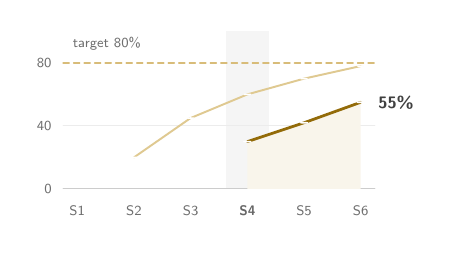
\begin{tikzpicture}[x=0.72cm,y=0.02cm,line cap=round,line join=round]
  \fill[black!4] (3.62,0) rectangle (4.38,100);
  \draw[gray!15,line width=0.3pt] (0.75,40) -- (6.25,40);
  \draw[amber!55,line width=0.5pt,dash pattern=on 2.2pt off 1.6pt] (0.75,80) -- (6.25,80);
  \draw[gray!40,line width=0.4pt] (0.75,0) -- (6.25,0);
  \ytick{0}{0}\ytick{40}{40}\ytick{80}{80}
  \node[anchor=south west,font=\sffamily\fontsize{5}{5}\selectfont,text=fog] at (0.75,82) {target 80\%};
  \fill[amber!8] (4,0) -- (4,30) -- (5,42) -- (6,55) -- (6,0) -- cycle;
  \draw[amber!45,line width=0.7pt] (2,20)--(3,45)--(4,60)--(5,70)--(6,78);
  \foreach \s/\v in {2/20,3/45,4/60,5/70,6/78}{\filldraw[fill=amber!45,draw=white,line width=0.5pt] (\s,\v) circle (0.055);}
  \draw[amber!80!black,line width=1pt] (4,30)--(5,42)--(6,55);
  \foreach \s/\v in {4/30,5/42,6/55}{\filldraw[fill=amber!80!black,draw=white,line width=0.5pt] (\s,\v) circle (0.062);}
  \node[anchor=west,font=\sffamily\fontsize{6}{6}\selectfont\bfseries,text=black!75] at (6.14,55) {55\%};
  \foreach \s in {1,2,3,5,6}{\node[anchor=north,yshift=-2.5pt,font=\sffamily\fontsize{5}{5}\selectfont,text=fog] at (\s,0) {S\s};}
  \node[anchor=north,yshift=-2.5pt,font=\sffamily\fontsize{5}{5}\selectfont\bfseries,text=black!60] at (4,0) {S4};
\end{tikzpicture}\\[0.5pt]
{\scriptsize\color{fog}\textcolor{amber!45}{\rule[0.5ex]{0.9em}{1.2pt}}\,syllable\quad \textcolor{amber!80!black}{\rule[0.5ex]{0.9em}{1.2pt}}\,word (CVC)}
\end{minipage}
\end{goalbox}

% ================= 3. Auto flags =================
\begin{notebox}
{\sffamily\scriptsize\bfseries\color{amber!60!black} AUTO FLAGS}\hspace{0.5em}{\small
Goal 1 and Goal 2 are on trajectory for their S8 targets (Goal 1: +8--10 pts/session since the S4 probe; Goal 2: 8/10 with 2 words planned for S7). \textbf{Goal 3 word-level accuracy (55\%) is below the linear trajectory to 80\%}: errors concentrate on back-vowel CVC (40\%); recommend increasing /s/+back-vowel practice density in S7 activities \ding{172}\ding{174} (rocket theme: \emph{sun}; review \emph{sock, suit}) --- flagged for the SOAP-note plan.}
\end{notebox}

% ================= 4. Clinician notes =================
\section{Clinician Notes \hspace{0.4em}{\normalfont\sffamily\scriptsize\color{black!55}(review of auto-compiled data; appended to the SOAP note)}}

\begin{tcolorbox}[colback=white,colframe=gray!30,boxrule=0.4pt,arc=2pt,
  left=8pt,right=8pt,top=6pt,bottom=6pt,boxsep=0pt,height=1.0cm]
\color{gray!45}\scriptsize\sffamily engagement / cue-level changes / observations not captured by counts \ldots
\end{tcolorbox}

\vfill
{\color{accentlt}\rule{\linewidth}{0.6pt}}\\[1pt]
{\scriptsize\color{black!55}\sffamily This is an illustrative example. Counts, accuracies and trends are for design demonstration only and cannot support clinical decision-making. SATE --- Record $\cdot$ Processing $\cdot$ Report.}

\end{document}
